% Options for packages loaded elsewhere
\PassOptionsToPackage{unicode}{hyperref}
\PassOptionsToPackage{hyphens}{url}
%
\documentclass[
  man]{apa6}
\usepackage{amsmath,amssymb}
\usepackage{iftex}
\ifPDFTeX
  \usepackage[T1]{fontenc}
  \usepackage[utf8]{inputenc}
  \usepackage{textcomp} % provide euro and other symbols
\else % if luatex or xetex
  \usepackage{unicode-math} % this also loads fontspec
  \defaultfontfeatures{Scale=MatchLowercase}
  \defaultfontfeatures[\rmfamily]{Ligatures=TeX,Scale=1}
\fi
\usepackage{lmodern}
\ifPDFTeX\else
  % xetex/luatex font selection
\fi
% Use upquote if available, for straight quotes in verbatim environments
\IfFileExists{upquote.sty}{\usepackage{upquote}}{}
\IfFileExists{microtype.sty}{% use microtype if available
  \usepackage[]{microtype}
  \UseMicrotypeSet[protrusion]{basicmath} % disable protrusion for tt fonts
}{}
\makeatletter
\@ifundefined{KOMAClassName}{% if non-KOMA class
  \IfFileExists{parskip.sty}{%
    \usepackage{parskip}
  }{% else
    \setlength{\parindent}{0pt}
    \setlength{\parskip}{6pt plus 2pt minus 1pt}}
}{% if KOMA class
  \KOMAoptions{parskip=half}}
\makeatother
\usepackage{xcolor}
\usepackage{graphicx}
\makeatletter
\def\maxwidth{\ifdim\Gin@nat@width>\linewidth\linewidth\else\Gin@nat@width\fi}
\def\maxheight{\ifdim\Gin@nat@height>\textheight\textheight\else\Gin@nat@height\fi}
\makeatother
% Scale images if necessary, so that they will not overflow the page
% margins by default, and it is still possible to overwrite the defaults
% using explicit options in \includegraphics[width, height, ...]{}
\setkeys{Gin}{width=\maxwidth,height=\maxheight,keepaspectratio}
% Set default figure placement to htbp
\makeatletter
\def\fps@figure{htbp}
\makeatother
\setlength{\emergencystretch}{3em} % prevent overfull lines
\providecommand{\tightlist}{%
  \setlength{\itemsep}{0pt}\setlength{\parskip}{0pt}}
\setcounter{secnumdepth}{-\maxdimen} % remove section numbering
% Make \paragraph and \subparagraph free-standing
\ifx\paragraph\undefined\else
  \let\oldparagraph\paragraph
  \renewcommand{\paragraph}[1]{\oldparagraph{#1}\mbox{}}
\fi
\ifx\subparagraph\undefined\else
  \let\oldsubparagraph\subparagraph
  \renewcommand{\subparagraph}[1]{\oldsubparagraph{#1}\mbox{}}
\fi
\newlength{\cslhangindent}
\setlength{\cslhangindent}{1.5em}
\newlength{\csllabelwidth}
\setlength{\csllabelwidth}{3em}
\newlength{\cslentryspacingunit} % times entry-spacing
\setlength{\cslentryspacingunit}{\parskip}
\newenvironment{CSLReferences}[2] % #1 hanging-ident, #2 entry spacing
 {% don't indent paragraphs
  \setlength{\parindent}{0pt}
  % turn on hanging indent if param 1 is 1
  \ifodd #1
  \let\oldpar\par
  \def\par{\hangindent=\cslhangindent\oldpar}
  \fi
  % set entry spacing
  \setlength{\parskip}{#2\cslentryspacingunit}
 }%
 {}
\usepackage{calc}
\newcommand{\CSLBlock}[1]{#1\hfill\break}
\newcommand{\CSLLeftMargin}[1]{\parbox[t]{\csllabelwidth}{#1}}
\newcommand{\CSLRightInline}[1]{\parbox[t]{\linewidth - \csllabelwidth}{#1}\break}
\newcommand{\CSLIndent}[1]{\hspace{\cslhangindent}#1}
\ifLuaTeX
\usepackage[bidi=basic]{babel}
\else
\usepackage[bidi=default]{babel}
\fi
\babelprovide[main,import]{english}
% get rid of language-specific shorthands (see #6817):
\let\LanguageShortHands\languageshorthands
\def\languageshorthands#1{}
% Manuscript styling
\usepackage{upgreek}
\captionsetup{font=singlespacing,justification=justified}

% Table formatting
\usepackage{longtable}
\usepackage{lscape}
% \usepackage[counterclockwise]{rotating}   % Landscape page setup for large tables
\usepackage{multirow}		% Table styling
\usepackage{tabularx}		% Control Column width
\usepackage[flushleft]{threeparttable}	% Allows for three part tables with a specified notes section
\usepackage{threeparttablex}            % Lets threeparttable work with longtable

% Create new environments so endfloat can handle them
% \newenvironment{ltable}
%   {\begin{landscape}\centering\begin{threeparttable}}
%   {\end{threeparttable}\end{landscape}}
\newenvironment{lltable}{\begin{landscape}\centering\begin{ThreePartTable}}{\end{ThreePartTable}\end{landscape}}

% Enables adjusting longtable caption width to table width
% Solution found at http://golatex.de/longtable-mit-caption-so-breit-wie-die-tabelle-t15767.html
\makeatletter
\newcommand\LastLTentrywidth{1em}
\newlength\longtablewidth
\setlength{\longtablewidth}{1in}
\newcommand{\getlongtablewidth}{\begingroup \ifcsname LT@\roman{LT@tables}\endcsname \global\longtablewidth=0pt \renewcommand{\LT@entry}[2]{\global\advance\longtablewidth by ##2\relax\gdef\LastLTentrywidth{##2}}\@nameuse{LT@\roman{LT@tables}} \fi \endgroup}

% \setlength{\parindent}{0.5in}
% \setlength{\parskip}{0pt plus 0pt minus 0pt}

% Overwrite redefinition of paragraph and subparagraph by the default LaTeX template
% See https://github.com/crsh/papaja/issues/292
\makeatletter
\renewcommand{\paragraph}{\@startsection{paragraph}{4}{\parindent}%
  {0\baselineskip \@plus 0.2ex \@minus 0.2ex}%
  {-1em}%
  {\normalfont\normalsize\bfseries\itshape\typesectitle}}

\renewcommand{\subparagraph}[1]{\@startsection{subparagraph}{5}{1em}%
  {0\baselineskip \@plus 0.2ex \@minus 0.2ex}%
  {-\z@\relax}%
  {\normalfont\normalsize\itshape\hspace{\parindent}{#1}\textit{\addperi}}{\relax}}
\makeatother

\makeatletter
\usepackage{etoolbox}
\patchcmd{\maketitle}
  {\section{\normalfont\normalsize\abstractname}}
  {\section*{\normalfont\normalsize\abstractname}}
  {}{\typeout{Failed to patch abstract.}}
\patchcmd{\maketitle}
  {\section{\protect\normalfont{\@title}}}
  {\section*{\protect\normalfont{\@title}}}
  {}{\typeout{Failed to patch title.}}
\makeatother

\usepackage{xpatch}
\makeatletter
\xapptocmd\appendix
  {\xapptocmd\section
    {\addcontentsline{toc}{section}{\appendixname\ifoneappendix\else~\theappendix\fi\\: #1}}
    {}{\InnerPatchFailed}%
  }
{}{\PatchFailed}
\keywords{Trace metal, Depression\newline\indent Word count: X}
\DeclareDelayedFloatFlavor{ThreePartTable}{table}
\DeclareDelayedFloatFlavor{lltable}{table}
\DeclareDelayedFloatFlavor*{longtable}{table}
\makeatletter
\renewcommand{\efloat@iwrite}[1]{\immediate\expandafter\protected@write\csname efloat@post#1\endcsname{}}
\makeatother
\usepackage{csquotes}
\usepackage{colortbl}
\ifLuaTeX
  \usepackage{selnolig}  % disable illegal ligatures
\fi
\IfFileExists{bookmark.sty}{\usepackage{bookmark}}{\usepackage{hyperref}}
\IfFileExists{xurl.sty}{\usepackage{xurl}}{} % add URL line breaks if available
\urlstyle{same}
\hypersetup{
  pdftitle={Correlation of trace metal and Depression},
  pdfauthor={Hao Chen},
  pdflang={en-EN},
  pdfkeywords={Trace metal, Depression},
  hidelinks,
  pdfcreator={LaTeX via pandoc}}

\title{Correlation of trace metal and Depression}
\author{Hao Chen\textsuperscript{}}
\date{}


\shorttitle{SHORT TITLE}

\authornote{

The authors made the following contributions. Hao Chen: Conceptualization, Writing - Original Draft Preparation, Writing - Review \& Editing.

}

\affiliation{\vspace{0.5cm}\textsuperscript{1} University of Chicago}

\abstract{%
One or two sentences providing a \textbf{basic introduction} to the field, comprehensible to a scientist in any discipline.
Two to three sentences of \textbf{more detailed background}, comprehensible to scientists in related disciplines.
One sentence clearly stating the \textbf{general problem} being addressed by this particular study.
One sentence summarizing the main result (with the words ``\textbf{here we show}'' or their equivalent).
Two or three sentences explaining what the \textbf{main result} reveals in direct comparison to what was thought to be the case previously, or how the main result adds to previous knowledge.
One or two sentences to put the results into a more \textbf{general context}.
Two or three sentences to provide a \textbf{broader perspective}, readily comprehensible to a scientist in any discipline.
}



\begin{document}
\maketitle

\hypertarget{introduction}{%
\section{Introduction}\label{introduction}}

Major Depressive Disorder (MDD) is a prevalent yet severe mood condition marked by experience of low mood and negative emotions for a long period of time(American Psychiatric Association, 2013). In 2019, approximately 280 million individuals, which includes 5\% of the adult population, were estimated to have experienced depression({``{GBD Results},''} n.d.). According to the statistics from the United States National Institute of Mental Health, around 21.0 million adults in the United States experienced at least one major depressive episode, accounting for 8.3\% of all U.S. adults({``Major {Depression} - {National Institute} of {Mental Health} ({NIMH}),''} n.d.).
MDD is a multifaceted and intricate condition, which can result in impairment of psychosocial functioning and quality of life(Saragoussi et al., 2018). In addition to depressed feelings, patients with MDD may experience a wide range of physical and cognitive symptoms, including feelings of sadness, irritability, loss of interest or pleasure in activities, changes in appetite or weight, sleep disturbances, fatigue, feelings of worthlessness or guilt, difficulty concentrating, and thoughts of death or suicide(American Psychiatric Association, 2013).
Etiology of MDD includes biological, environmental, and personal vulnerabilities(National Research Council (US) and Institute of Medicine (US) Committee on Depression, England, \& Sim, 2009). Lately, there has been growing attention towards metallomic research in psychiatry, with a focus on examining the involvement of essential trace elements in both the development and progression of MDD symptoms. An essential trace element refers to a mineral or dietary element necessary in small amounts for an organism's proper growth, development, and physiology(Bowen, 1966). These elements are vital for conducting essential metabolic activities in organisms. Examples of essential trace metals in human nutrition include Na, K, Mg, Ca, Fe, Mn, Co, Cu, Zn and Mo(Zoroddu et al., 2019). The trace metals play important catalytic and structural roles. These elements facilitate essential biochemical reactions by serving as cofactors for numerous enzymes and as stabilizing agents for the structures of enzymes and proteins(Prashanth, Kattapagari, Chitturi, Baddam, \& Prasad, 2015). Alterations in the accumulation or absence of these components can trigger alternative metabolic pathways, potentially contributing to various neurodevelopmental diseases and conditions (Yui, 2016).
Baj et al.~(2013) conducted an narrative review of the relationship between levels of selected trace elements in the serum of individuals with MDD and the initiation and advancement of this mental health disorder(Baj et al., 2023). Findings of this review reveal that the levels of metal content in the body are related to the outcomes of individuals with MDD in various ways. For example, Li et al.~(2020) has demonstrated that elevated levels of copper can disrupt the functioning of NMDA receptors, contributing to cognitive deficits in MDD(Li et al., 2020). Increased copper concentrations can also impair AMPA receptor function, leading to disruptions in glutamatergic transmission, supporting the Glu hypothesis of depression(Gerhard, Wohleb, \& Duman, 2016; Peters et al., 2011; Styczeń et al., 2017).
Although there relationship between the trace metals in human serum and MDD has been widely studied, there are limited research on the results of trace metal and how they relate to the frequency of MDD symptom. This study aims to reveal the relationship between the two.

\begin{table}
\centering
\caption{\label{tab:racial-demographic}Racial Demographics}
\centering
\resizebox{\ifdim\width>\linewidth\linewidth\else\width\fi}{!}{
\begin{tabular}[t]{l|r}
\hline
Var1 & Freq\\
\hline
\cellcolor{gray!10}{Mexican American} & \cellcolor{gray!10}{263}\\
\hline
Non-Hispanic Asian & 262\\
\hline
\cellcolor{gray!10}{Non-Hispanic Black} & \cellcolor{gray!10}{430}\\
\hline
Non-Hispanic White & 636\\
\hline
\cellcolor{gray!10}{Other} & \cellcolor{gray!10}{104}\\
\hline
Other Hispanic & 164\\
\hline
\end{tabular}}
\end{table}

\hypertarget{methods}{%
\section{Methods}\label{methods}}

\hypertarget{dataset}{%
\subsection{Dataset}\label{dataset}}

This research employs a cross-sectional methodology, leveraging data from the National Health and Nutrition Examination Survey (NHANES) conducted by the US National Center for Health Statistics. Objectives of the survey encompass evaluating the health and nutritional conditions of individuals across the United States, as well as identifying the prevalence of significant diseases and their risk contributors. The NHANES database includes a wide array of information, such as demographic specifics, nutritional insights, results from physical exams, laboratory test results, participant questionnaire answers, and confidential data.

\hypertarget{participants}{%
\subsection{Participants}\label{participants}}

Participants aged 3 to 5 years, along with a one-third subset of those aged 6 and above, were considered eligible for this study. Due to privacy concerns, access to urine lead data for the 3 to 5 age group and urine strontium and uranium data for those aged 3 and above is restricted to the NCHS Research Data Center. However, the dataset does include urine lead data for participants aged 6 and older, as well as urine barium, cadmium, cesium, cobalt, manganese, molybdenum, antimony, thallium, tin, and tungsten for all eligible participants aged 3 and above. For further details on accessing urine lead, strontium, and uranium data, refer to the Analytic Notes.

\hypertarget{description-of-laboratory-methodology-for-trace-metal}{%
\subsection{Description of Laboratory Methodology for Trace Metal}\label{description-of-laboratory-methodology-for-trace-metal}}

This technique accurately quantifies various metals in urine samples by utilizing mass spectrometry, preceded by a straightforward dilution preparation of the samples. The process begins with the introduction of liquid specimens into the mass spectrometer via an inductively coupled plasma (ICP) ionization source. Here, a nebulizer converts the sample into fine droplets within an argon gas stream. These droplets then proceed into the ICP, where they are ionized. The ions navigate through a focusing area, enter the dynamic reaction cell (DRC), pass through the quadrupole mass filter, and ultimately, the detector sequentially counts them in rapid succession. This method enables the precise identification of individual isotopes for each element analyzed.

\hypertarget{detection-limits-for-trace-metal}{%
\subsection{Detection Limits for Trace Metal}\label{detection-limits-for-trace-metal}}

The detection limits remained uniform across all analytes within the dataset. For each analyte, two specific variables are furnished. A variable name ending with ``LC'' (for example, URDUBALC) signifies if the measurement fell below the detection limits : a ``0'' value indicates the measurement was at or above this limits, whereas a ``1'' denotes it was below. Conversely, the variable starting with URX (for example, URXUBA) reports the actual measurement for the analyte. When the measurement for an analyte is below the detection limit (for instance, URDUBALC=1), a predetermined substitute value is used in its place. This substitute value is calculated as the detection limit divided by the square root of 2.

\hypertarget{depression-assessment}{%
\subsection{Depression Assessment}\label{depression-assessment}}

The assessment of participants' depressive symptoms was conducted using the Patient Health Questionnaire-9 (PHQ-9), a nine-item instrument designed for depression screening. The PHQ-9 is recognized as a reliable and validated method for detecting common depression and related disorders, especially in primary care environments(Kim, Choi, Lim, \& Hong, 2016). This questionnaire includes nine prompts, with responses scored based on the Diagnostic and Statistical Manual of Mental Disorders (DSM) criteria as follows: 0 (``Never''), 1 (``A few days''), 2 (``More than a week''), and 3 (``Almost every day''), leading to a total possible score between 0 and 27. A score within the 0-9 range is considered indicative of a non-depressive state, whereas a score of 10 or higher suggests the presence of depression. The PHQ-9 has demonstrated high sensitivity (0.88) and specificity (0.85) for identifying depression at a threshold score of 10 or above(Levis, Benedetti, \& Thombs, 2019).

\hypertarget{data-analysis}{%
\subsection{Data analysis}\label{data-analysis}}

We used R (Version 4.3.2; R Core Team, 2023) and the R-packages \emph{dplyr} (Version 1.1.4; Wickham, François, Henry, Müller, \& Vaughan, 2023), \emph{ggplot2} (Version 3.5.0; Wickham, 2016), \emph{kableExtra} (Version 1.4.0; Zhu, 2024), \emph{knitr} (Version 1.45; Xie, 2015), \emph{papaja} (Version 0.1.2; Aust \& Barth, 2023), \emph{readr} (Version 2.1.5; Wickham, Hester, \& Bryan, 2024), and \emph{tinylabels} (Version 0.2.4; Barth, 2023) for all our analyses.

This is a plot showing the correlation of LCsum and DPQsum. As shown in the plot \ref{fig:LCDPQ-plot}, we see\ldots{}

\begin{figure}
\centering
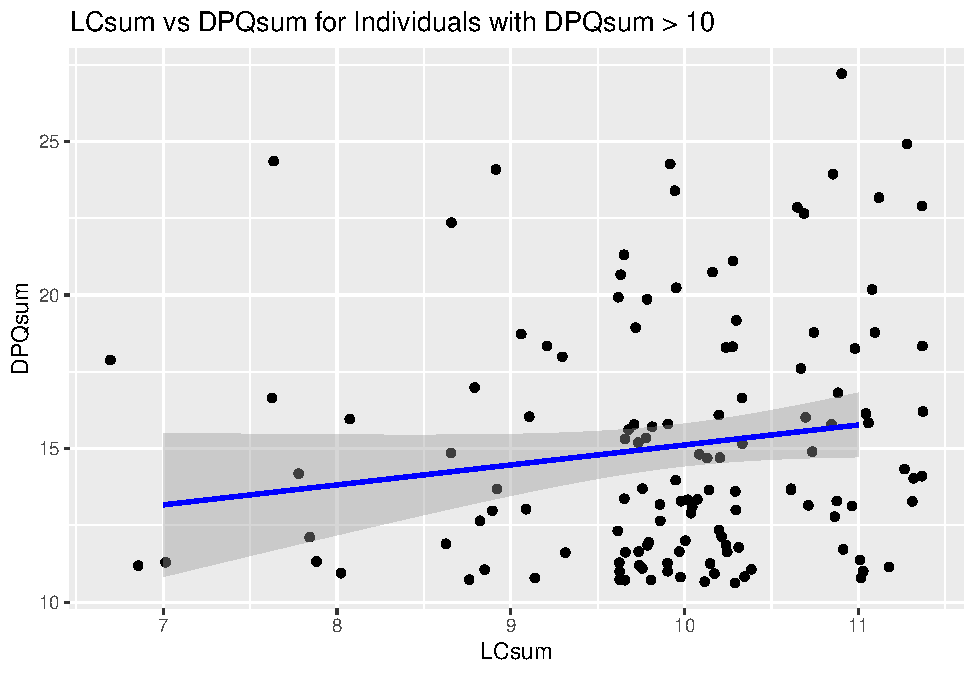
\includegraphics{nhanes2017_files/figure-latex/LCDPQ-plot-1.pdf}
\caption{\label{fig:LCDPQ-plot}LCsum vs DPQsum for Individuals with DPQsum \textgreater{} 10}
\end{figure}

\begin{verbatim}
## Warning in cor.test.default(LCDPQ_data$LCsum, LCDPQ_data$DPQsum, method =
## "spearman"): Cannot compute exact p-value with ties
\end{verbatim}

The spearman test result for the type of trace metal exceed detection limits and the frequency of depression symptom is c(S = 293916.316865034), NULL, 0.0430328503343255, c(rho = 0.178453944362047), c(rho = 0), two.sided, Spearman's rank correlation rho, LCDPQ\_data\(LCsum and LCDPQ_data\)DPQsum

\begin{verbatim}
## Warning in cor.test.default(LCDPQ_data[[var]], LCDPQ_data$DPQsum, method =
## "spearman"): Cannot compute exact p-value with ties

## Warning in cor.test.default(LCDPQ_data[[var]], LCDPQ_data$DPQsum, method =
## "spearman"): Cannot compute exact p-value with ties

## Warning in cor.test.default(LCDPQ_data[[var]], LCDPQ_data$DPQsum, method =
## "spearman"): Cannot compute exact p-value with ties

## Warning in cor.test.default(LCDPQ_data[[var]], LCDPQ_data$DPQsum, method =
## "spearman"): Cannot compute exact p-value with ties

## Warning in cor.test.default(LCDPQ_data[[var]], LCDPQ_data$DPQsum, method =
## "spearman"): Cannot compute exact p-value with ties

## Warning in cor.test.default(LCDPQ_data[[var]], LCDPQ_data$DPQsum, method =
## "spearman"): Cannot compute exact p-value with ties

## Warning in cor.test.default(LCDPQ_data[[var]], LCDPQ_data$DPQsum, method =
## "spearman"): Cannot compute exact p-value with ties

## Warning in cor.test.default(LCDPQ_data[[var]], LCDPQ_data$DPQsum, method =
## "spearman"): Cannot compute exact p-value with ties

## Warning in cor.test.default(LCDPQ_data[[var]], LCDPQ_data$DPQsum, method =
## "spearman"): Cannot compute exact p-value with ties

## Warning in cor.test.default(LCDPQ_data[[var]], LCDPQ_data$DPQsum, method =
## "spearman"): Cannot compute exact p-value with ties

## Warning in cor.test.default(LCDPQ_data[[var]], LCDPQ_data$DPQsum, method =
## "spearman"): Cannot compute exact p-value with ties
\end{verbatim}

\begin{verbatim}
##    Min. 1st Qu.  Median    Mean 3rd Qu.    Max. 
##   0.000   9.000  10.000   9.585  11.000  11.000
\end{verbatim}

\begin{verbatim}
##    Min. 1st Qu.  Median    Mean 3rd Qu.    Max. 
##   0.000   0.000   1.000   3.158   5.000  27.000
\end{verbatim}

Means of LCsum is 9.59, which means participants have an average of 9 or 10 types of trace metal above detection limits. For the same people group, their average score for frequency of depression symptom is 3.16.

\hypertarget{results}{%
\section{Results}\label{results}}

\hypertarget{discussion}{%
\section{Discussion}\label{discussion}}

\newpage

\hypertarget{references}{%
\section{References}\label{references}}

\hypertarget{refs}{}
\begin{CSLReferences}{1}{0}
\leavevmode\vadjust pre{\hypertarget{ref-americanpsychiatricassociationDiagnosticStatisticalManual2013}{}}%
American Psychiatric Association. (2013). \emph{Diagnostic and {Statistical Manual} of {Mental Disorders}} (Fifth Edition). {American Psychiatric Association}. \url{https://doi.org/10.1176/appi.books.9780890425596}

\leavevmode\vadjust pre{\hypertarget{ref-R-papaja}{}}%
Aust, F., \& Barth, M. (2023). \emph{{papaja}: {Prepare} reproducible {APA} journal articles with {R Markdown}}. Retrieved from \url{https://github.com/crsh/papaja}

\leavevmode\vadjust pre{\hypertarget{ref-bajTraceElementsLevels2023}{}}%
Baj, J., Bargieł, J., Cabaj, J., Skierkowski, B., Hunek, G., Portincasa, P., \ldots{} Smoleń, A. (2023). Trace {Elements Levels} in {Major Depressive Disorder}---{Evaluation} of {Potential Threats} and {Possible Therapeutic Approaches}. \emph{International Journal of Molecular Sciences}, \emph{24}(20), 15071. \url{https://doi.org/10.3390/ijms242015071}

\leavevmode\vadjust pre{\hypertarget{ref-R-tinylabels}{}}%
Barth, M. (2023). \emph{{tinylabels}: Lightweight variable labels}. Retrieved from \url{https://cran.r-project.org/package=tinylabels}

\leavevmode\vadjust pre{\hypertarget{ref-bowen1966trace}{}}%
Bowen, H. J. M. (1966). \emph{Trace elements in biochemistry}. {Academic Press}. Retrieved from \url{https://books.google.com/books?id=AH2T3X0enHkC}

\leavevmode\vadjust pre{\hypertarget{ref-GBDResults}{}}%
{GBD Results}. (n.d.). Retrieved February 27, 2024, from \url{https://vizhub.healthdata.org/gbd-results}

\leavevmode\vadjust pre{\hypertarget{ref-gerhardEmergingTreatmentMechanisms2016}{}}%
Gerhard, D. M., Wohleb, E. S., \& Duman, R. S. (2016). Emerging treatment mechanisms for depression: Focus on glutamate and synaptic plasticity. \emph{Drug Discovery Today}, \emph{21}(3), 454--464. \url{https://doi.org/10.1016/j.drudis.2016.01.016}

\leavevmode\vadjust pre{\hypertarget{ref-kimUrinaryPhthalateMetabolites2016}{}}%
Kim, K.-N., Choi, Y.-H., Lim, Y.-H., \& Hong, Y.-C. (2016). Urinary phthalate metabolites and depression in an elderly population: {National Health} and {Nutrition Examination Survey} 2005--2012. \emph{Environmental Research}, \emph{145}, 61--67. \url{https://doi.org/10.1016/j.envres.2015.11.021}

\leavevmode\vadjust pre{\hypertarget{ref-levisAccuracyPatientHealth2019}{}}%
Levis, B., Benedetti, A., \& Thombs, B. D. (2019). Accuracy of {Patient Health Questionnaire-9} ({PHQ-9}) for screening to detect major depression: Individual participant data meta-analysis. \emph{BMJ}, l1476. \url{https://doi.org/10.1136/bmj.l1476}

\leavevmode\vadjust pre{\hypertarget{ref-liAlleviationCognitiveDeficits2020}{}}%
Li, Z., Wang, G., Zhong, S., Liao, X., Lai, S., Shan, Y., \ldots{} Jia, Y. (2020). Alleviation of cognitive deficits and high copper levels by an {NMDA} receptor antagonist in a rat depression model. \emph{Comprehensive Psychiatry}, \emph{102}, 152200. \url{https://doi.org/10.1016/j.comppsych.2020.152200}

\leavevmode\vadjust pre{\hypertarget{ref-MajorDepressionNational}{}}%
Major {Depression} - {National Institute} of {Mental Health} ({NIMH}). (n.d.). Retrieved February 27, 2024, from \url{https://www.nimh.nih.gov/health/statistics/major-depression}

\leavevmode\vadjust pre{\hypertarget{ref-nationalresearchcouncilusandinstituteofmedicineuscommitteeondepressionEtiologyDepression2009}{}}%
National Research Council (US) and Institute of Medicine (US) Committee on Depression, P. P., England, M. J., \& Sim, L. J. (2009). The {Etiology} of {Depression}. In \emph{Depression in {Parents}, {Parenting}, and {Children}: {Opportunities} to {Improve Identification}, {Treatment}, and {Prevention}}. {National Academies Press (US)}. Retrieved from \url{https://www.ncbi.nlm.nih.gov/books/NBK215119/}

\leavevmode\vadjust pre{\hypertarget{ref-petersBiphasicEffectsCopper2011}{}}%
Peters, C., Muñoz, B., Sepúlveda, F. J., Urrutia, J., Quiroz, M., Luza, S., \ldots{} Opazo, C. (2011). Biphasic effects of copper on neurotransmission in rat hippocampal neurons. \emph{Journal of Neurochemistry}, \emph{119}(1), 78--88. \url{https://doi.org/10.1111/j.1471-4159.2011.07417.x}

\leavevmode\vadjust pre{\hypertarget{ref-prashanthReviewRoleEssential2015}{}}%
Prashanth, L., Kattapagari, K., Chitturi, R., Baddam, V. R., \& Prasad, L. (2015). A review on role of essential trace elements in health and disease. \emph{Journal of Dr. NTR University of Health Sciences}, \emph{4}(2), 75. \url{https://doi.org/10.4103/2277-8632.158577}

\leavevmode\vadjust pre{\hypertarget{ref-R-base}{}}%
R Core Team. (2023). \emph{R: A language and environment for statistical computing}. Vienna, Austria: R Foundation for Statistical Computing. Retrieved from \url{https://www.R-project.org/}

\leavevmode\vadjust pre{\hypertarget{ref-saragoussiLongtermFollowupHealthrelated2018}{}}%
Saragoussi, D., Christensen, M. C., Hammer-Helmich, L., Rive, B., Touya, M., \& Haro, J. M. (2018). Long-term follow-up on health-related quality of life in major depressive disorder: A 2-year {European} cohort study. \emph{Neuropsychiatric Disease and Treatment}, \emph{Volume 14}, 1339--1350. \url{https://doi.org/10.2147/NDT.S159276}

\leavevmode\vadjust pre{\hypertarget{ref-styczenSerumZincConcentration2017}{}}%
Styczeń, K., Sowa-Kućma, M., Siwek, M., Dudek, D., Reczyński, W., Szewczyk, B., \ldots{} Nowak, G. (2017). The serum zinc concentration as a potential biological marker in patients with major depressive disorder. \emph{Metabolic Brain Disease}, \emph{32}(1), 97--103. \url{https://doi.org/10.1007/s11011-016-9888-9}

\leavevmode\vadjust pre{\hypertarget{ref-R-ggplot2}{}}%
Wickham, H. (2016). \emph{ggplot2: Elegant graphics for data analysis}. Springer-Verlag New York. Retrieved from \url{https://ggplot2.tidyverse.org}

\leavevmode\vadjust pre{\hypertarget{ref-R-dplyr}{}}%
Wickham, H., François, R., Henry, L., Müller, K., \& Vaughan, D. (2023). \emph{Dplyr: A grammar of data manipulation}. Retrieved from \url{https://CRAN.R-project.org/package=dplyr}

\leavevmode\vadjust pre{\hypertarget{ref-R-readr}{}}%
Wickham, H., Hester, J., \& Bryan, J. (2024). \emph{Readr: Read rectangular text data}. Retrieved from \url{https://CRAN.R-project.org/package=readr}

\leavevmode\vadjust pre{\hypertarget{ref-R-knitr}{}}%
Xie, Y. (2015). \emph{Dynamic documents with {R} and knitr} (2nd ed.). Boca Raton, Florida: Chapman; Hall/CRC. Retrieved from \url{https://yihui.org/knitr/}

\leavevmode\vadjust pre{\hypertarget{ref-yuiEditorialThematicIssue2016}{}}%
Yui, K. (2016). Editorial ({Thematic Issue}: {New Therapeutic Targets} for {Autism Spectrum Disorders}). \emph{CNS \& Neurological Disorders - Drug Targets}, \emph{15}(5), 529--532. \url{https://doi.org/10.2174/1871527315999160502125423}

\leavevmode\vadjust pre{\hypertarget{ref-R-kableExtra}{}}%
Zhu, H. (2024). \emph{kableExtra: Construct complex table with 'kable' and pipe syntax}. Retrieved from \url{https://CRAN.R-project.org/package=kableExtra}

\leavevmode\vadjust pre{\hypertarget{ref-zorodduEssentialMetalsHumans2019}{}}%
Zoroddu, M. A., Aaseth, J., Crisponi, G., Medici, S., Peana, M., \& Nurchi, V. M. (2019). The essential metals for humans: A brief overview. \emph{Journal of Inorganic Biochemistry}, \emph{195}, 120--129. \url{https://doi.org/10.1016/j.jinorgbio.2019.03.013}

\end{CSLReferences}


\end{document}
